%!TEX root = ../../main.tex

\chapter{Modellhafte Darstellung zur Evaluierung}

\section{Versuchsaufbau}

\subsection{Motorenmodell}

\subsection{Hardwaremodell}
\label{subsec:hardwaremodell}

\section{Technische Umsetzung}

\subsection{Detektion des Propellerblattes}
\label{sec:detect_propeller}
Um neben einer Unwuchtdetektion auch eine Unwuchtlokalisierung zu ermöglichen, ist die Detektion mindestens eines Propellerblattes zwingend notwendig.
Für die Lokalisierung der Unwucht muss der Arduino die Unwuchtmessung jeweils pro vollständiger Umdrehung ($360^\circ$ Umdrehung) des Propellers starten.
Durch die Detektion beider Propellerblätter ergeben sich prinzipiell Vorteile bei der Zuordnung der Messergebnisse der Unwucht. 
Da sich dies jedoch, wie in den folgenden Kapiteln aufgezeigt wird, aufgrund der technischen Umsetzung als problematisch herausstellt und durch die Detektion eines Propellerblattes und der Umdrehungsgeschwindigkeit des Propellers Rückschlüsse auf das zweite Propellerblatt gezogen werden können, wird im Zuge dieser Studienarbeit auf die Detektion des zweiten Propellerblattes verzichtet.

\subsubsection*{Theoretische Vorgehensweise}
Für die Detektion des Propellerblattes werden zwei technische Lösungen erarbeitet, welche im späteren Verlauf dieses Kapitels gegenüber gestellt werden.
Beiden Lösungen liegt die gleiche theoretische Vorgehensweise zugrunde:
\begin{enumerate}
	\item Eine Seite des Propellers schwarz anmalen / schwarz bekleben
	\item Propeller mit definierter Drehzahl rotieren lassen
	\item Bei Detektion der schwarzen Fläche Interrupt auslösen
\end{enumerate}


\begin{figure}[h]
	\centering
	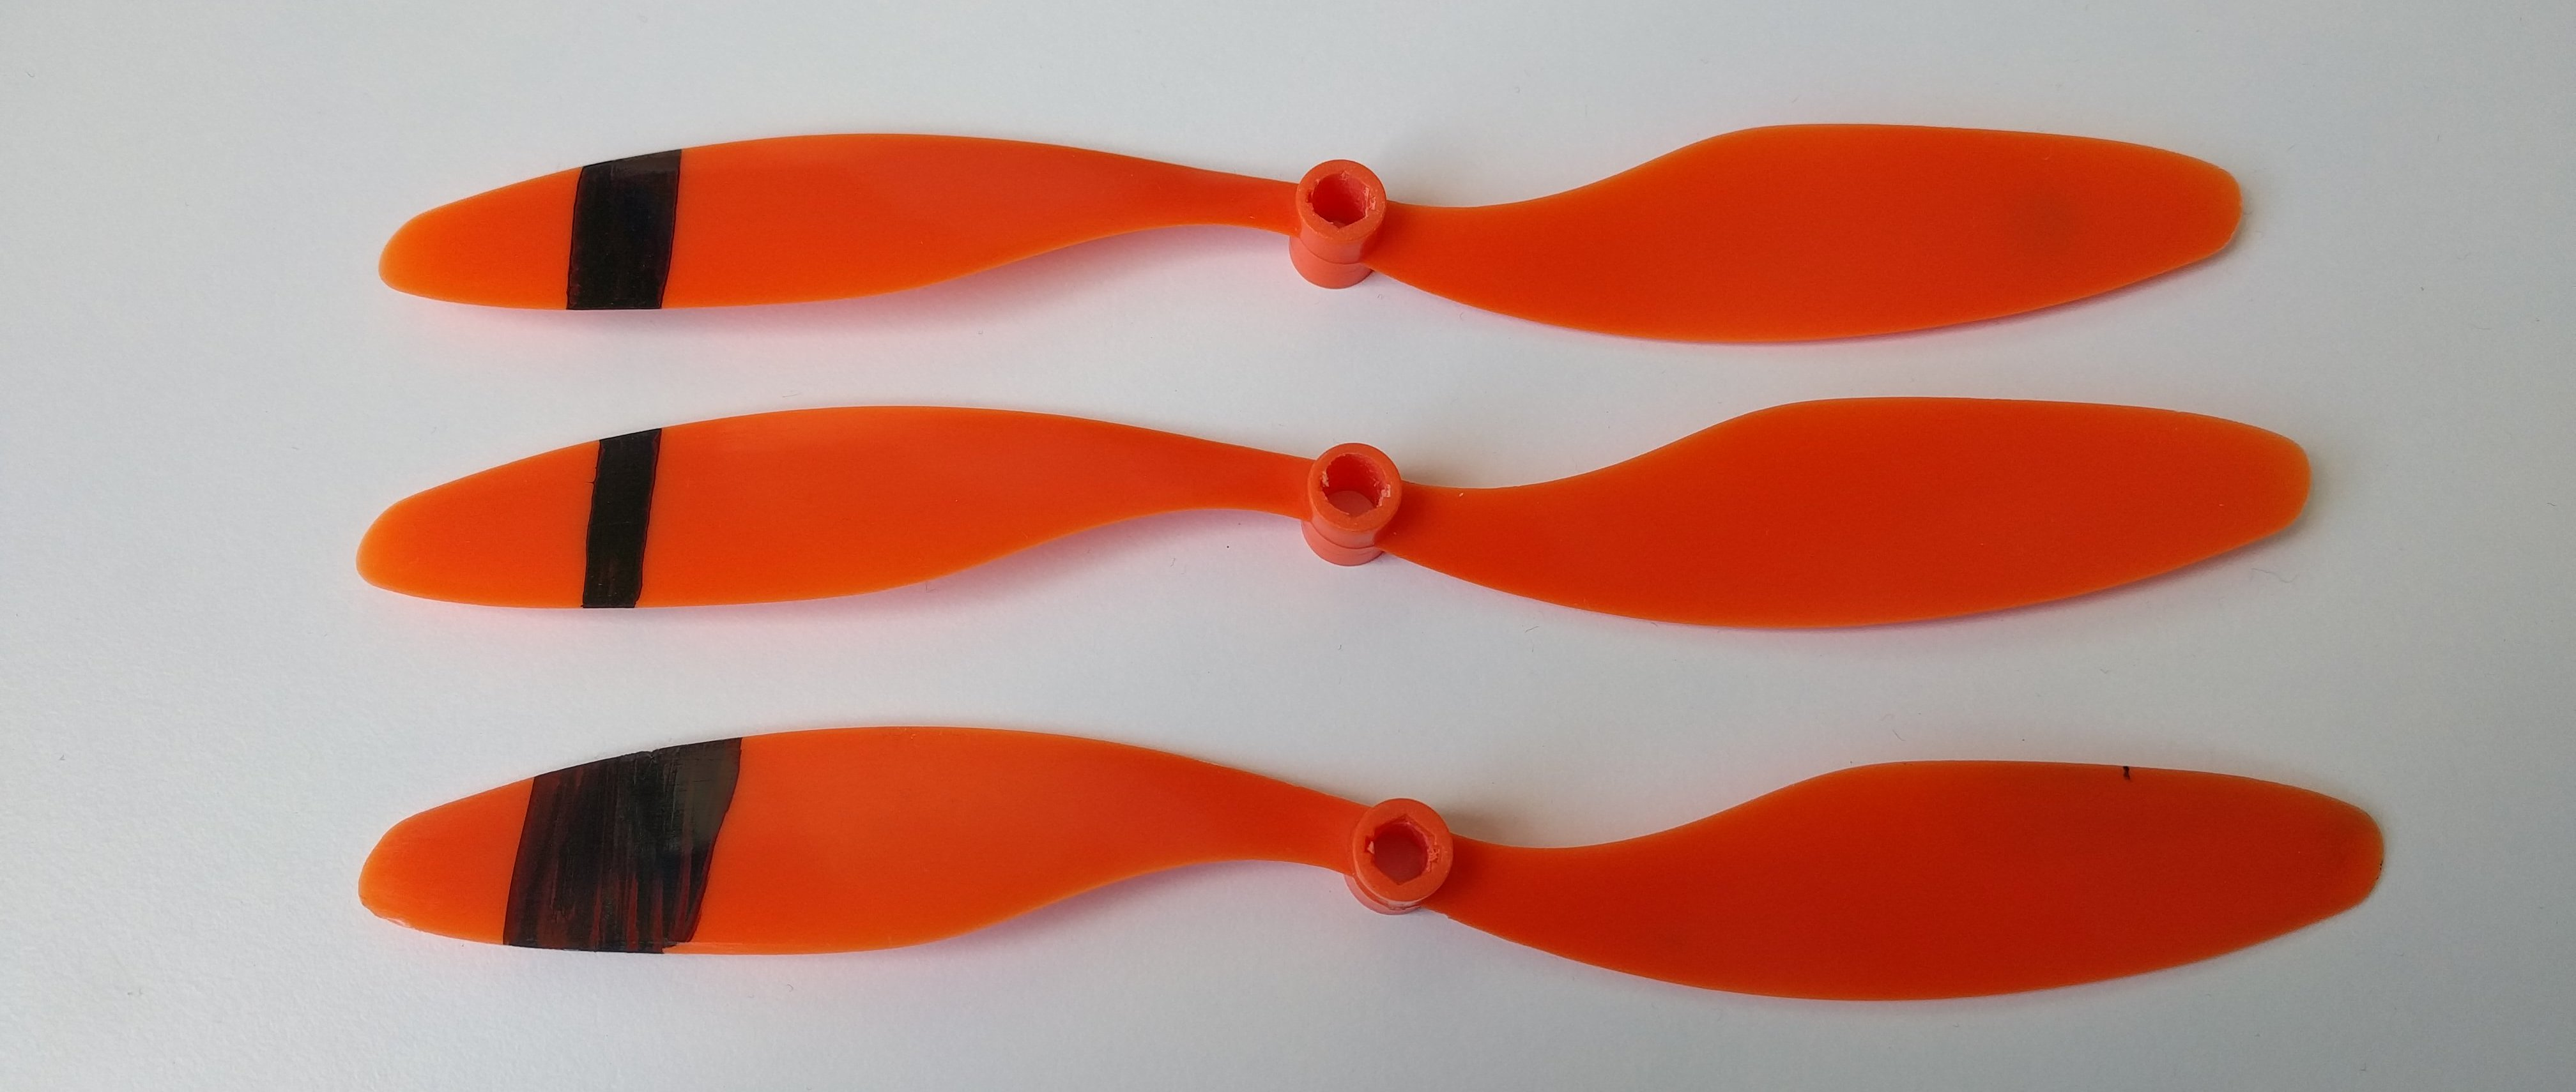
\includegraphics[width=.9\textwidth]{chapter/03/propeller_detektion.jpg}
	\caption{Modifikation zur Detektion eines Propellerblattes}
	\label{fig:propeller_detektion}
\end{figure}
Wie in Abbildung \ref{fig:propeller_detektion} erkennbar ist, gestaltet sich die Detektion des zweiten Propellerblattes als schwierig. 
Während das zweite Propellerblatt lediglich weiß markiert werden muss um dieses mithilfe des Lichtsensors zu detektieren, benötigt der \ac{IR} eine schwarz markierte Fläche.
Dies führt dazu, dass bei laufendem Motor zwar zwischen beiden Propellerblättern unterschieden werden kann (jedes zweite erkannte Propellerblatt ist das gleiche), jedoch keine verlässliche Aussage möglich ist, an welchem der beiden Propellerblätter die Unwucht auftritt, da eine eindeutige Unterscheidung zwischen den Propellerblättern durch den Sensor nicht möglich ist.

Treten beispielsweise durch Lichteinflüsse bedingte Messfehler auf, kann dies zu einem Überspringen bzw. Nichtdetektieren des Propellerblattes führen.
Wird die Messung mit nur einem markierten Propellerblatt durchgeführt und durch einen Messfehler nicht erkannt, ist die Messung bis zur nächsten Detektion prinzipiell falsch, kann aber später als Ausreißer ignoriert werden.
Wird die Messung mit beidseitig markierten Propellerblättern durchgeführt und ein Propellerblatt übersprungen, verschiebt sich die Position des Propellerblattes für die restliche Messung.
Dies würde zu einem vollkommen falschen Messergebnis führen.
Falsche Werte könnten nicht mehr als Ausreißer aussortiert werden, da diese ab dem Zeitpunkt des Messfehlers bis zum Zeitpunkt des nächsten Messfehlers bzw. bis zum Ende der Messung per se richtig wären, jedoch um 180$^\circ$ verschoben.

\subsubsection*{Vergleich zwischen Sensoren}
Zur Detektion des Propellerblattes stehen zwei verschiedene Arten an Sensoren zur Auswahl, welche im Folgenden gegenübergestellt und bewertet werden.

\newcolumntype{M}{>{\centering\arraybackslash}X}
\begin{table}[h]
	\centering
	\begin{tabularx}{0.95\textwidth}{M|M}

		Lichtsensor & IR-Reflektions-Sensor \\
		\hline
		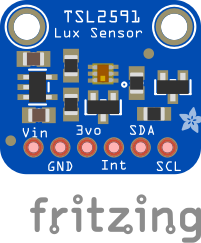
\includegraphics[height=3cm]{images/chapter/03/sensor_tsl2591.jpg} & 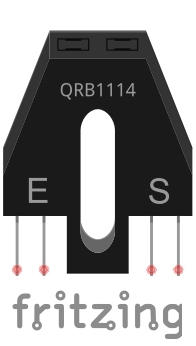
\includegraphics[height=4cm]{images/chapter/03/sensor_ir.jpg}  \\
		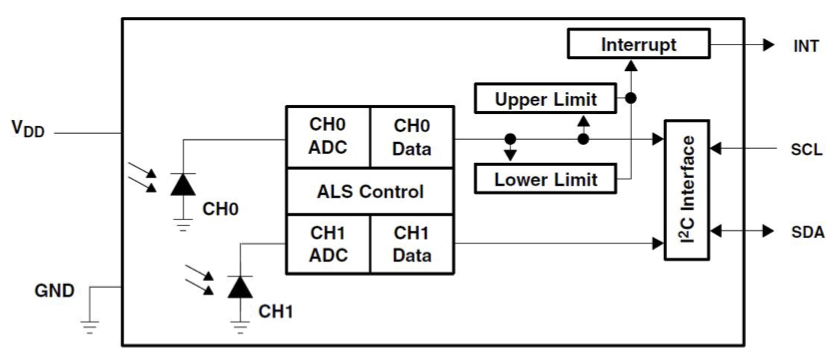
\includegraphics[height=3cm]{images/chapter/03/sensor_tsl2591_schema.png} & 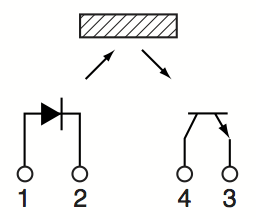
\includegraphics[height=3cm]{images/chapter/03/sensor_ir_schema.png} \\
		Adafruit TSL2591 & Adafruit Reflective IR Sensor \newline \\
	\end{tabularx}
	\caption{Vergleich zwischen zwei verschiedenen Arten an Sensoren zur Detektion des Propellerblattes}
\end{table}

Wie bereits beschrieben, erfolgt die Detektion des Propellerblattes bei beiden Sensoren durch die Detektion einer schwarzen Fläche.
Die technologischen Unterschiede der beiden Sensoren, beeinflussen die Einsetzbarkeit im Kontext dieser Studienarbeit in diversen Aspekten, welche im Folgenden dargestellt werden.
Neben der Differenzierung zwischen infrarotem Lichtspektrum und sichtbarem Lichtspektrum bei der Messung, weist der Lichtsensor eine hohe Lux-Reichweite auf \cite[S.1]{tsl2591_datasheet}.
\begin{figure}[H]
	\centering
	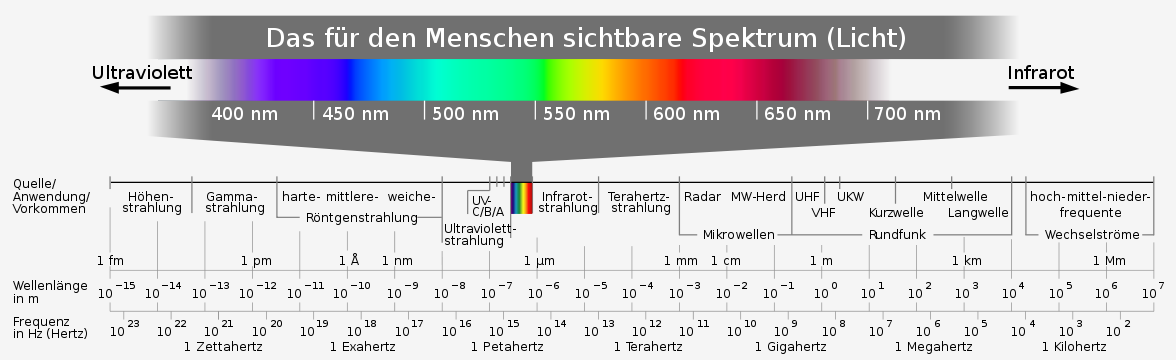
\includegraphics[width=\textwidth]{images/chapter/03/lichtspektrum.png}
	\caption{Darstellung des gesamten Lichtspektrums \cite[]{light_spectrum}}
\end{figure}
Hierduch können unerwünschte Lichteinflüsse, wie beispielsweise helle Sonneinstrahlung, vermieden werden.
Dies erlaubt den Einsatz des Lichtsensors in nahezu allen Lichtverhältnissen - ein nicht zu vernachlässigender Aspekt, da hierdurch die Unwuchtmessung am realen Flugzeugmotor nicht zwingend in einer Umgebung mit kontrollierbaren Lichteinflüssen wie beispielsweise einem Hangar stattfinden muss.
Des Weiteren bietet der Lichtsensor eine integrierte Interrupt-Schnittstelle, wodurch die Komplexität deutlich reduziert werden kann im Vergleich zu einem \ac{IR}.
Trotz der Tatsache, dass der Lichtsensor in den soeben beschriebenen Aspekten einem \ac{IR} deutlich überlegen ist, bietet ein \ac{IR} Vorteile, welche letztlich ausschlaggebend sind für die Entscheidung, welcher der beiden Sensoren verwendet werden soll.
Der wichtigste Aspekt hierbei ist die deutlich höhere Abtastrate des \ac{IR} im Vergleich zum Lichtsensor. 
\begin{figure}[H]
	\centering
	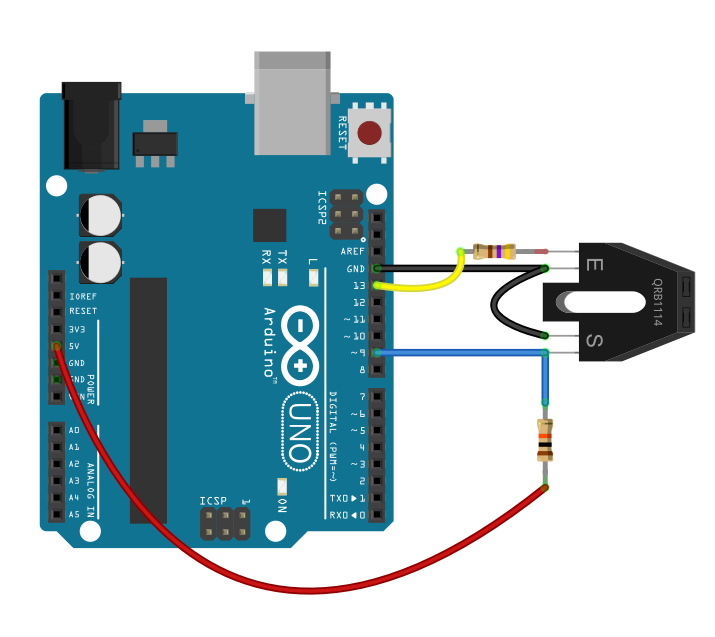
\includegraphics[width=0.75\textwidth]{images/chapter/03/sensor_ir_schaltung.png}
	\caption{Beispielhafte Verwendung des \ac{IR}s \cite{sensor_ir_schaltung}}
	\label{fig:ir_example}
\end{figure}
Abbildung \ref{fig:ir_example} stellt einen exemplarischen Verwendungszweck des \ac{IR}s dar. 
Der Sensor (in Abbildung \ref{fig:ir_example} durch ein S repräsentiert) ist sowohl direkt mit dem Arduino, als auch mit einem Pull-Up-Widerstand verbunden.
Dies hat zur Folge, dass am Port des Arduinos 5\ac{V} anliegen, solange der Sensor eine Reflexion des vom Emitter (in Abbildung \ref{fig:ir_example} durch ein E repräsentiert) ausgesendeten Lichtes erhält.
Wird das Licht nicht reflektiert - dies ist der Fall sobald sich die schwarze Fläche des Propellerblattes vor dem \ac{IR} befindet - liegt am Arduino Port 0\ac{V} an.
Für die Detektion des Propellerplattes, respektive für den Wechsel zwischen 5\ac{V} und 0\ac{V} (wird auch als Rise bzw. Fall-Time bezeichnet) benötigt der \ac{IR} lediglich eine Zeit von 8$\mu$s ausgehend einer Temperatur von 25$^\circ$C \cite[S.2]{ir_datasheet}.
Der Lichtsensor hingegen integriert alle gemessenen Werte über einen zuvor definierten Zeitraum.
Das Problem hierbei ist, dass für die Dauer des Zeitraumes lediglich folgende Werte verwendet werden können \cite[S.13]{tsl2591_datasheet}:
\begin{itemize}
	\item 100ms
	\item 200ms
	\item 300ms
	\item 400ms
	\item 500ms
	\item 600ms
\end{itemize}
Ein Flugzeugmotor dreht im Leerlauf mit ca. 2500 U/min.
FÜr ein valides Ergebnis, muss die minimale Abtastrate höher als die maximale Umdrehungszahl des Motors sein, um sicherzustellen, dass der schwarz markierte Bereich des Propellerblattes auch detektiert wurde.
Umgerechnet bedeutet dies, dass der Propeller für eine Umdrehung ca. 24ms benötigt.
\begin{equation}
2500\;U/min \approx 42\;U/s \approx 1\;U/\,24\;ms
\label{equation_revolutions}
\end{equation}
Da die geringste Abtastrate 100ms beträgt, ist der Lichtsensor für den Anwendugsfall dieser Studienarbeit ungeeignet.
Aus diesem Grund wird für die Umsetzung dieser Studienarbeit auf den \ac{IR} als Sensor zur Detektion des Propellerblattes gesetzt.

\subsubsection*{Probleme bei der Detektion des Propellerblattes mit einem \ac{IR}}
Aufgrund der technischen Beschaffenheit des \ac{IR}s ist eine Detektion des Propellerblattes in der Theorie ohne Weiteres möglich.
Die Praxis zeigt allerdings, dass hierbei einige Probleme auftreten können.

Ein Problem ist die Positionierung des \ac{IR}s.
Dieser benötigt einen Abstand zwischen Sensor und Propellerblatt von minimal 2mm bis maximal 10mm \cite[Description]{sensor_ir_description}.
Des Weiteren ist der passende Winkel zum Propellerblatt für eine erfolgreiche Detektion entscheidend.
Es ist nicht ausreichend, den Sensor permanent an einer Stelle zu befestigen, da sich durch die Zentrifugalkräfte der gewichteten Propellerblätter (Gewichte werden verwendet um Unwucht zu erzeugen - hierauf wird in Kapitel \ref{subsec:detektion_der_unwucht} genauer eingegangen) der Abstand zwischen Propellerblatt und Sensor verändert.
\begin{figure}[H]
	\centering
	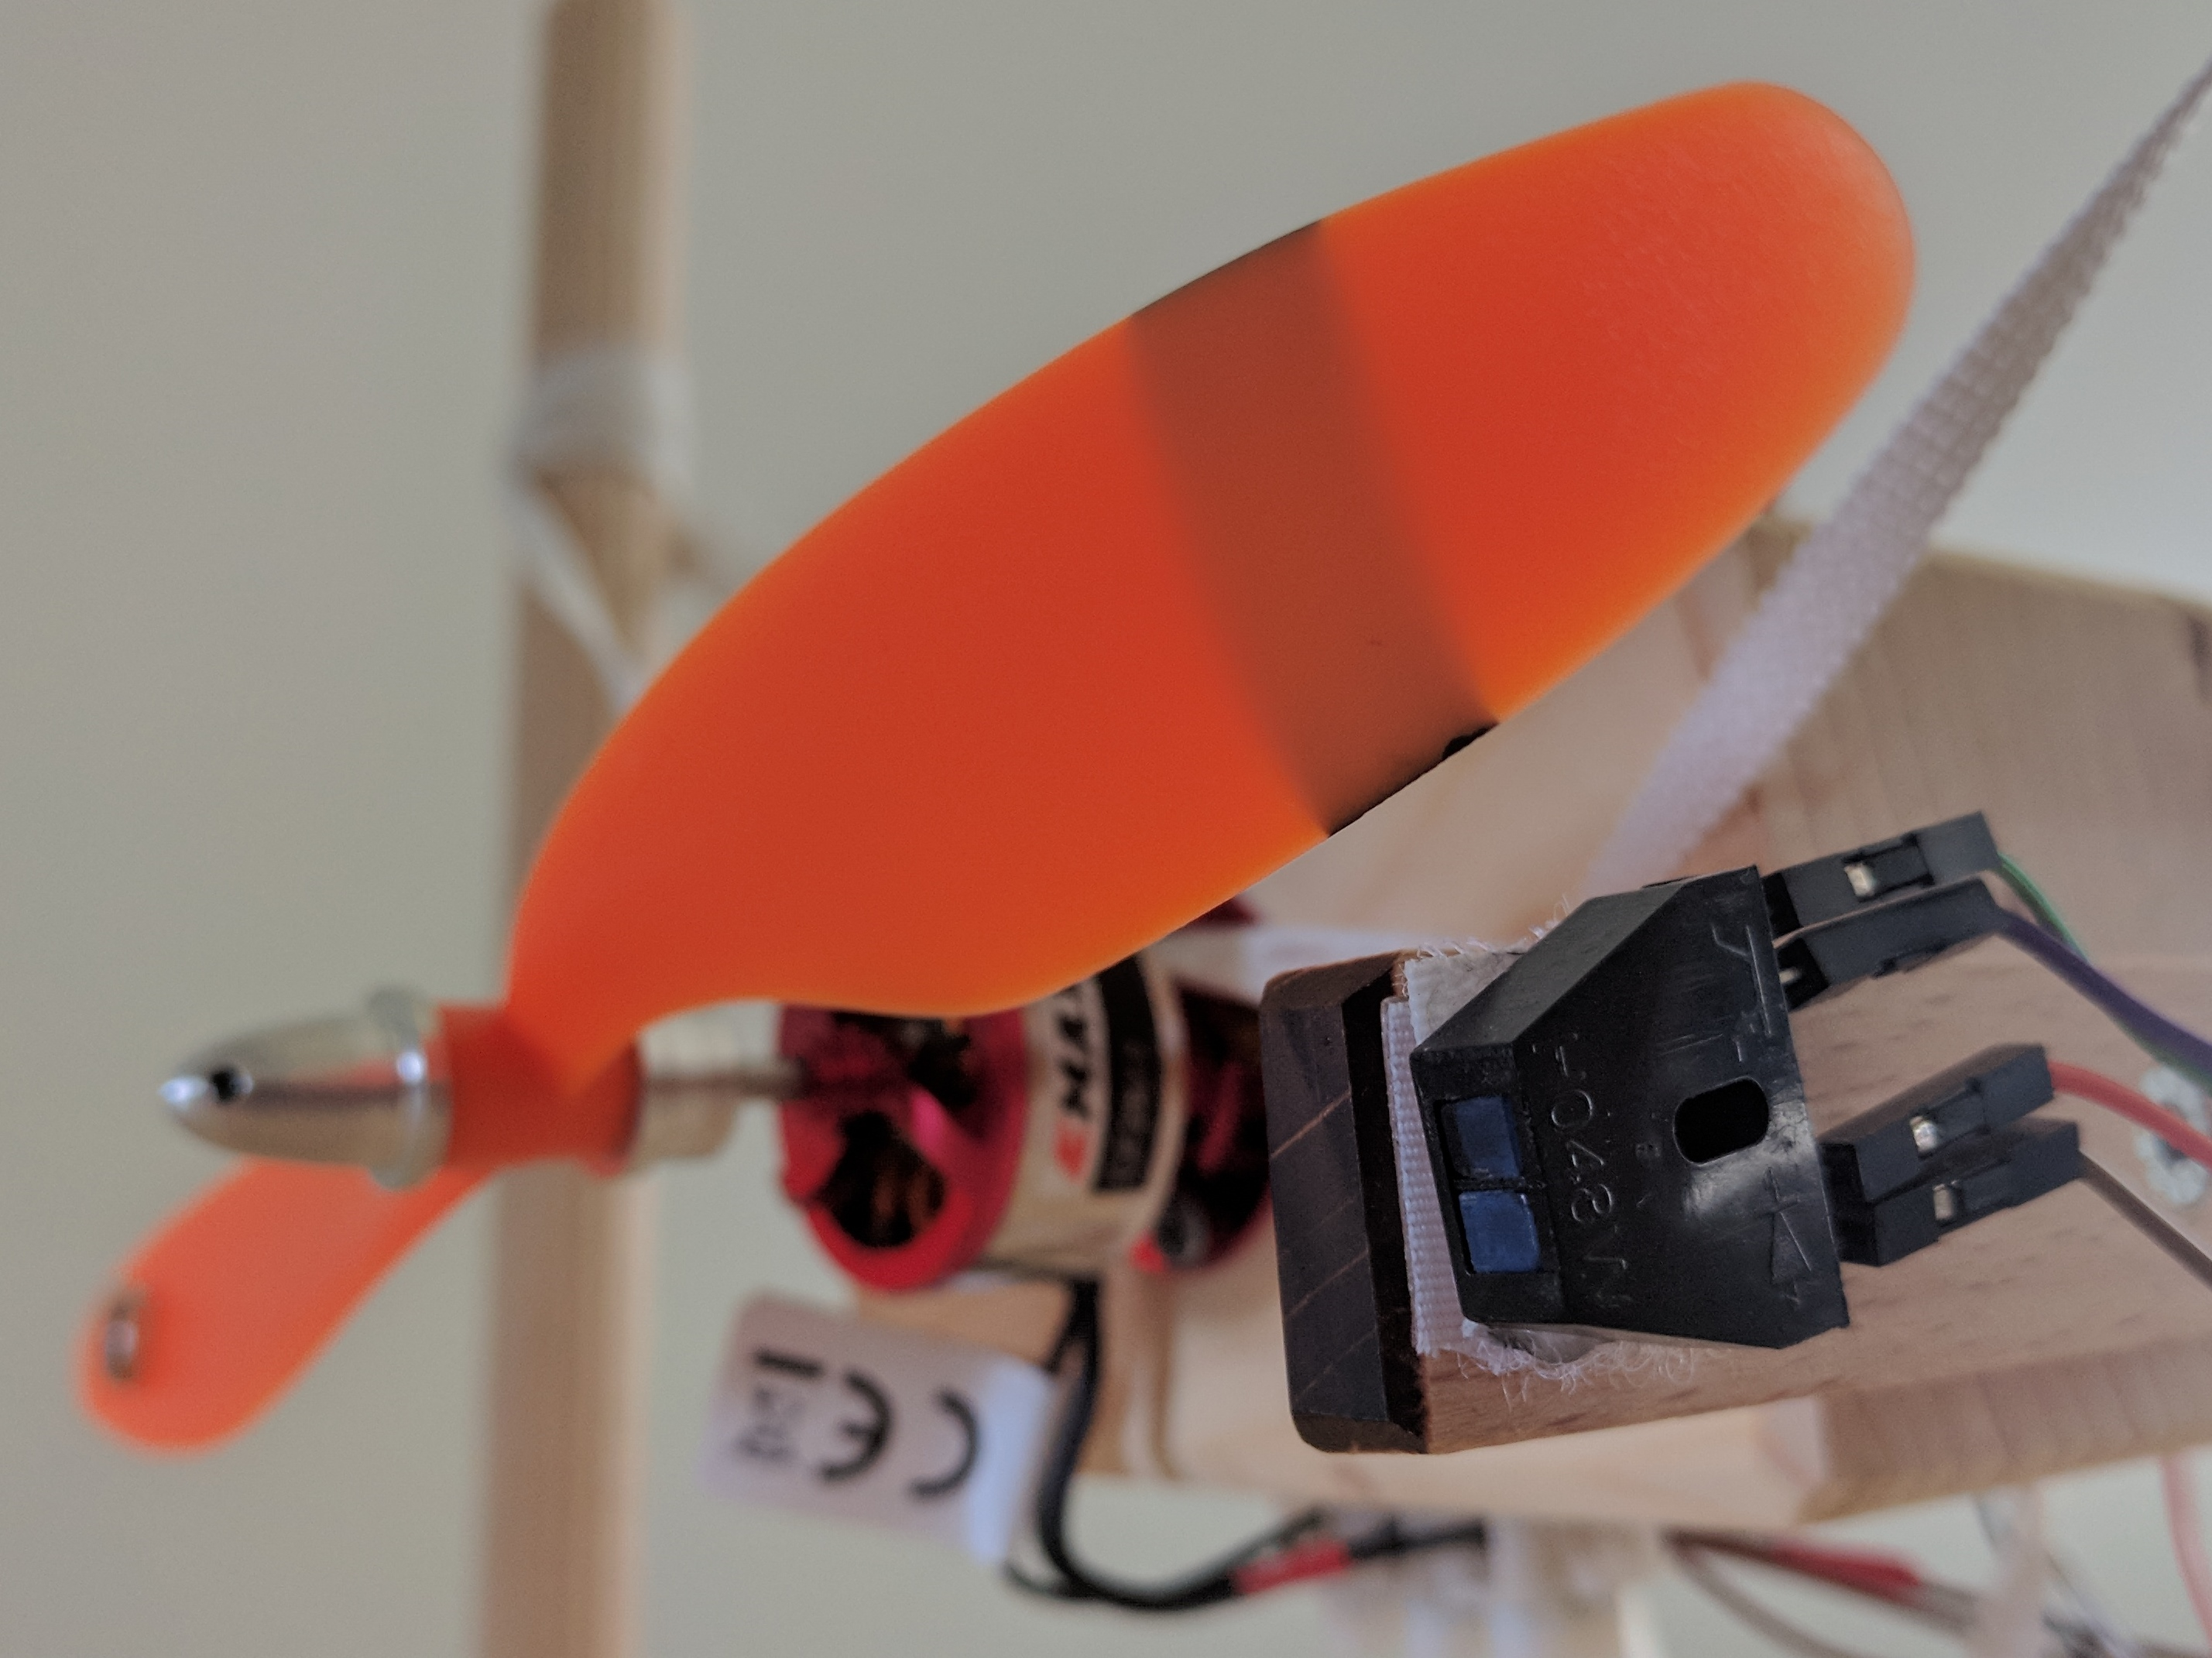
\includegraphics[width=0.9\textwidth]{images/chapter/03/exp_ir_sensor.jpg}
	\caption{Befestigung des Sensors mithilfe eines Klettbandes}
	\label{fig:exp_ir_sensor}
\end{figure}
Aus diesem Grund wird die Holzkonstruktion mit einem Klettband versehen, wie in Abbildung \ref{fig:exp_ir_sensor} zu sehen ist.
Dies ermöglicht es, den Sensor für jeden Propeller individuell einzustellen.

Neben dem Abstand bzw. dem Winkel des \ac{IR}s spielen Lichteinflüsse eine Rolle.
Im Gegensatz zum Lichtsensor ist der \ac{IR} trotz einer zusätzlichen Schutzkappe anfälliger gegenüber auf den Sensor einströmendes Licht \cite[Features]{ir_datasheet}.
Dies hat zur Folge, dass der Versuch nur in einer Umgebung mit kontrollierten Lichteinflüssen erfolgreich stattfinden kann.
Auffällig ist dieses Phänomen, sobald sich der Sensor direkt vor einem Fenster mit Blickrichtung auf dieses befindet.
Zu geringes Licht ist ein weiteres Problem, da hier die schwarze Fläche des Propellerblattes durch den \ac{IR} nicht mehr zuverlässig detektiert werden kann.

Das größte Problem stellt die Kombination eines \ac{9-DOF} Sensors und \ac{IR}s an einem einzigen Arduino dar.
\begin{figure}[H]
	\centering
	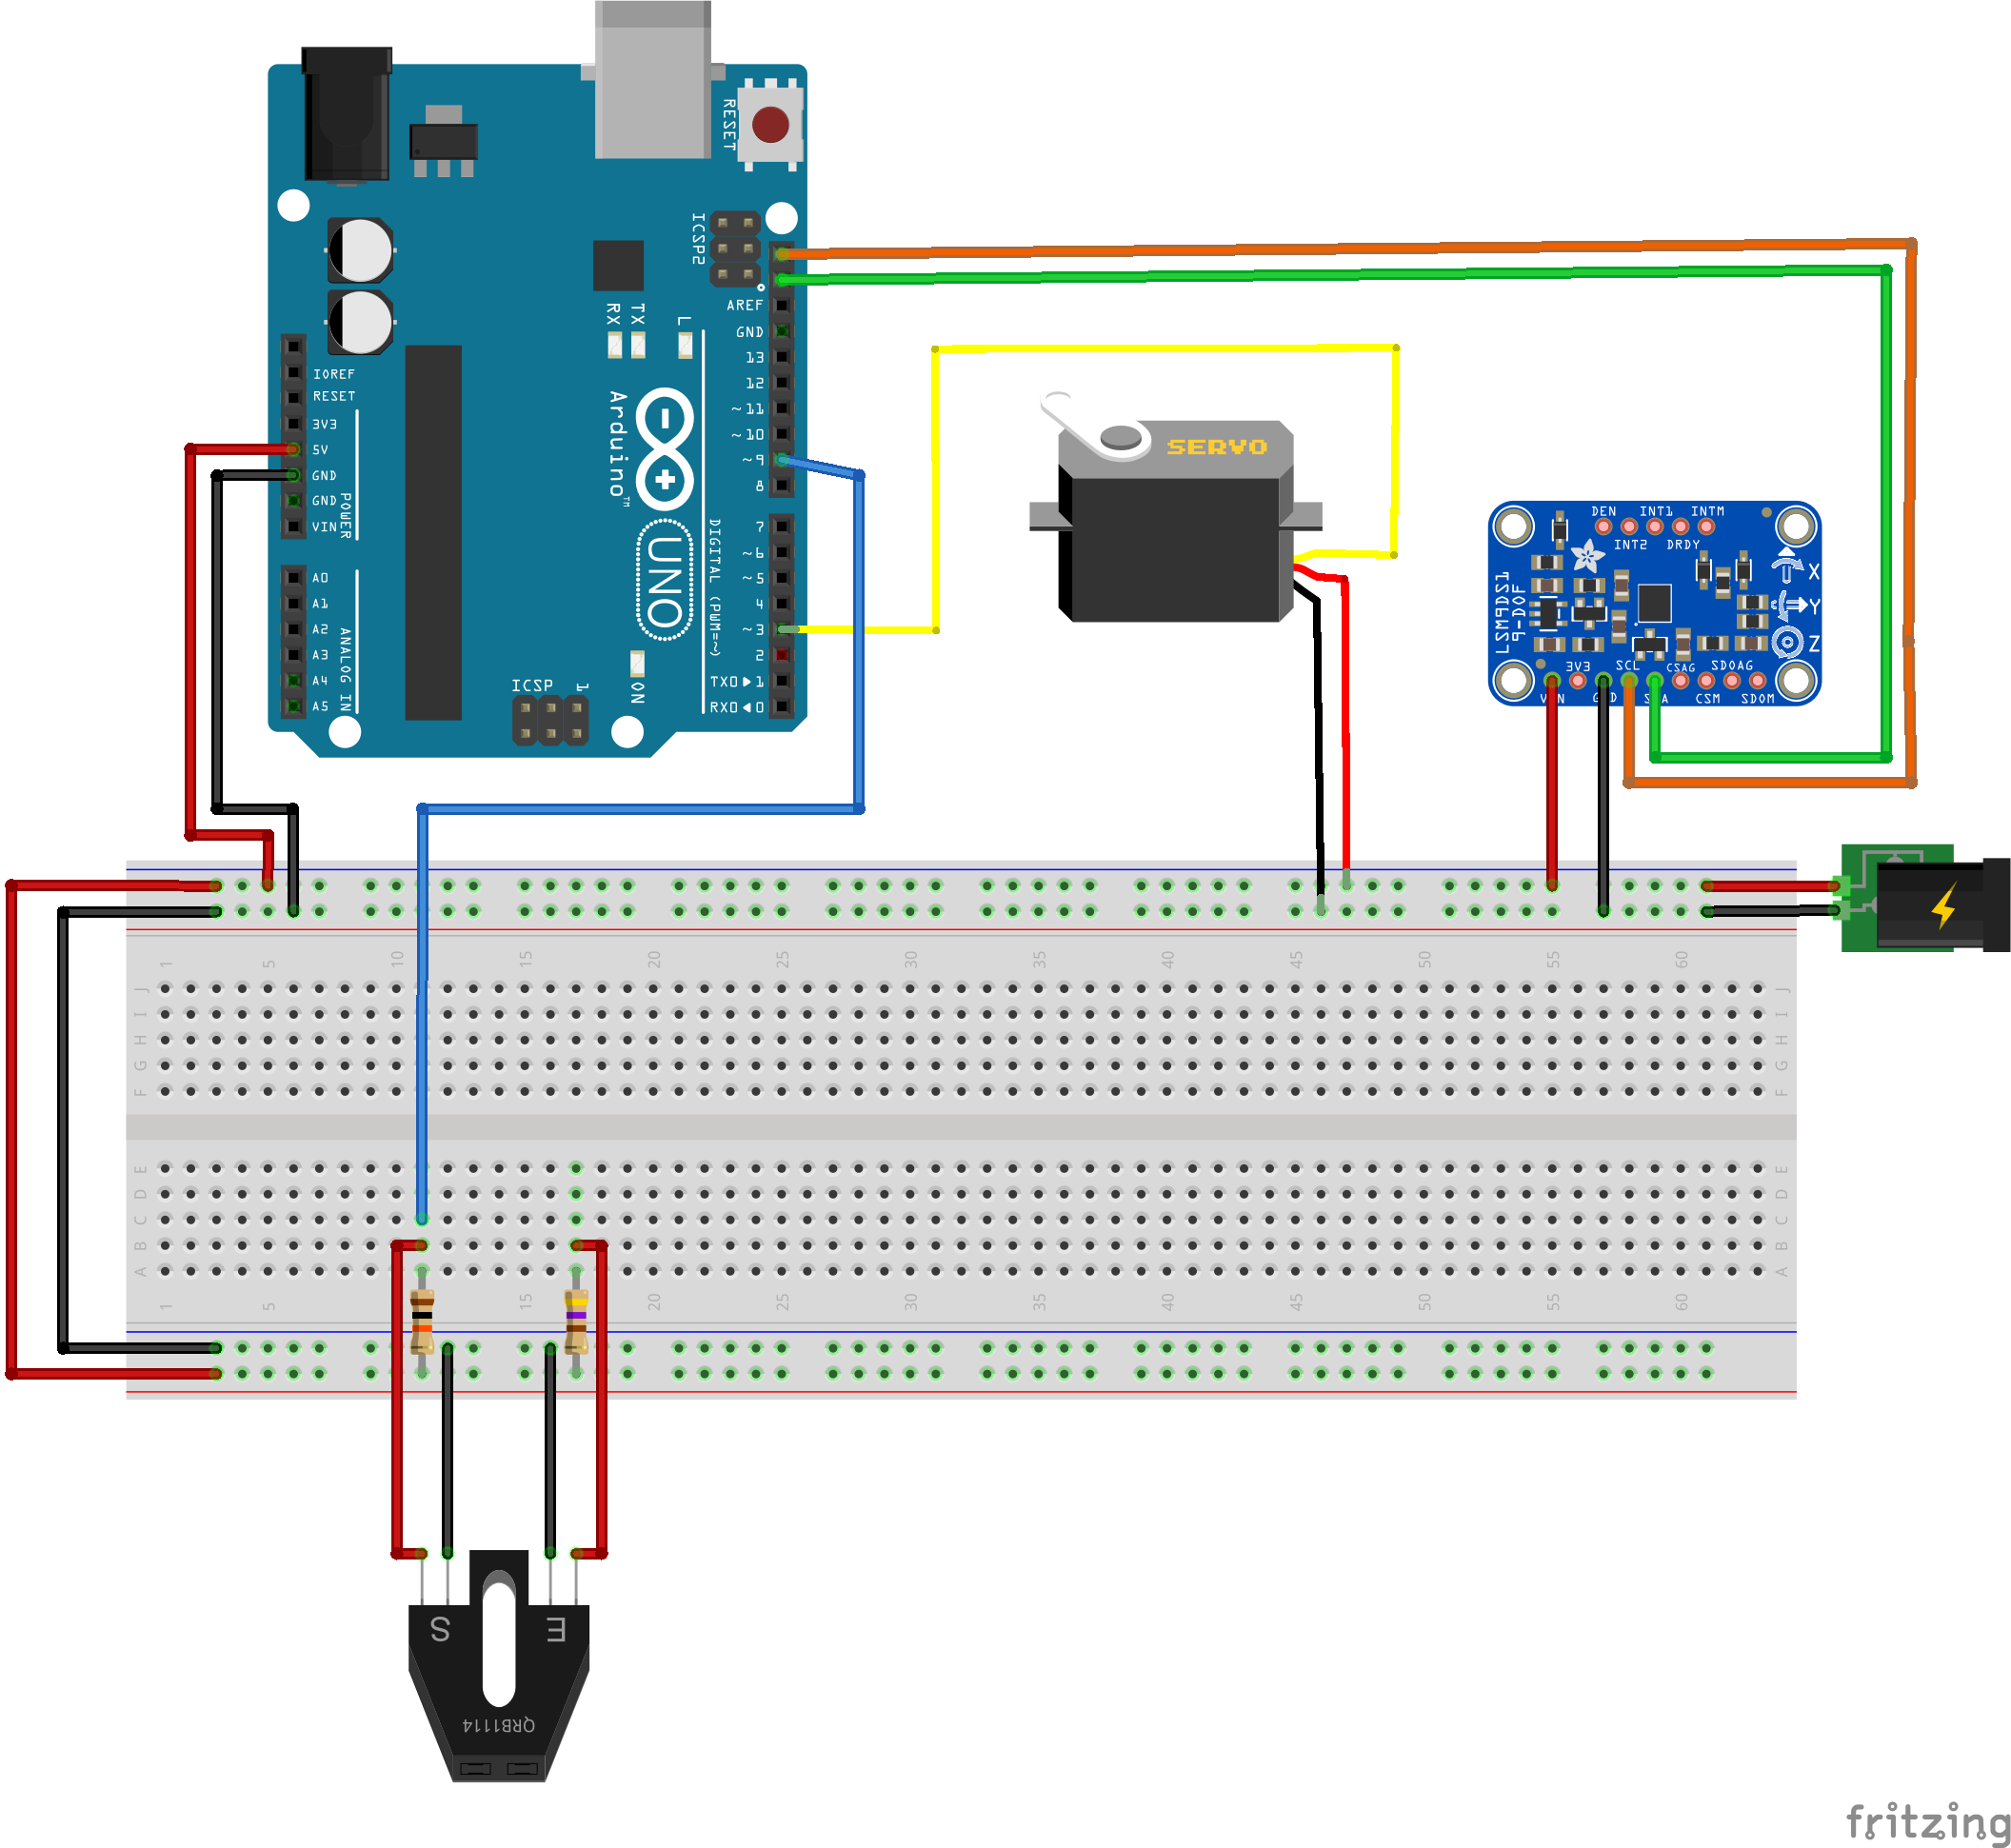
\includegraphics[width=0.9\textwidth]{images/chapter/03/hardware-layout-with-one-arduino.png}
	\caption{Altes Hardwaremodell mit einem Arduino}
\end{figure}
Bei gleichzeitigem Messen beider Sensoren ist eine zuverlässige Detektion des Rotorblattes nicht möglich.
Abbildung \ref{fig:interrupts_are_shit} stellt die Messergebnisse des \ac{IR}s graphisch dar.
\begin{figure}[H]
	\centering
	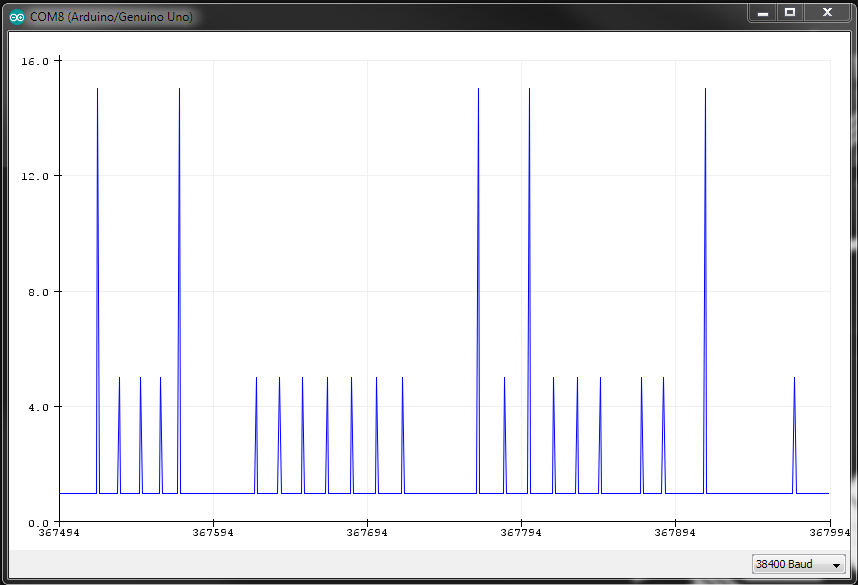
\includegraphics[width=0.9\textwidth]{images/chapter/03/interrupts_are_shit.png}
	\caption{Messwerte des \ac{IR}s bei gleichzeitiger Messung eines \ac{IR}s und eines \ac{9-DOF}s}
	\label{fig:interrupts_are_shit}
\end{figure}
Wie in Abbildung \ref{fig:interrupts_are_shit} zu erkennen ist, wird das Propellerblatt nur unregelmäßig erkannt.
Des Weiteren werden teilweise 3 Interrupts durch die \ac{ISR} erkannt.

Aus diesem Grund erfolgt eine Aufteilung der Sensoren auf die zwei Arduinos \ac{A1} und \ac{A2} wie in Abbildung \todo{ref auf hardwaremodell bild setzen} dargestellt. 
Weiterhin erfolgt eine Aufgabenteilung, wie in Abbildung \ref{fig:aufgaben-arduinos} dargestellt.
\begin{figure}[H]
	\centering
	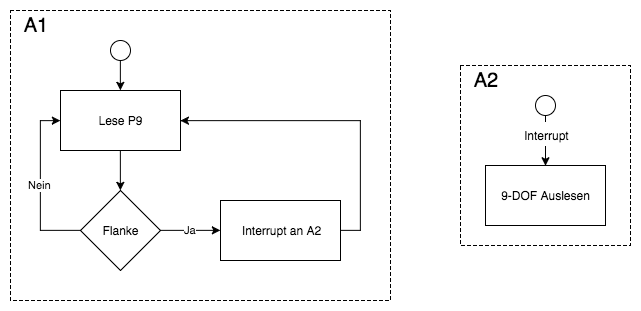
\includegraphics[width=0.9\textwidth]{images/chapter/03/aufgaben-arduinos.png}
	\caption{Aufgaben der beiden Arduinos \ac{A1} und \ac{A2}}
	\label{fig:aufgaben-arduinos}
\end{figure}
Durch die Trennung beider Sensoren und die Aufgabenteilung in Propellerblattdetektion und Unwuchtmessung ist \ac{A1} in der Lage das Propellerblatt konstant (im Rahmen einer gewissen Fehlertoleranz) zu detektieren.
Für ein besseres Verständnis, kann der Programmablauf von \ac{A1} dem Anhang \ref{lst:arduino_selfmade_interrupts} entnommen werden.
\begin{figure}[H]
	\centering
	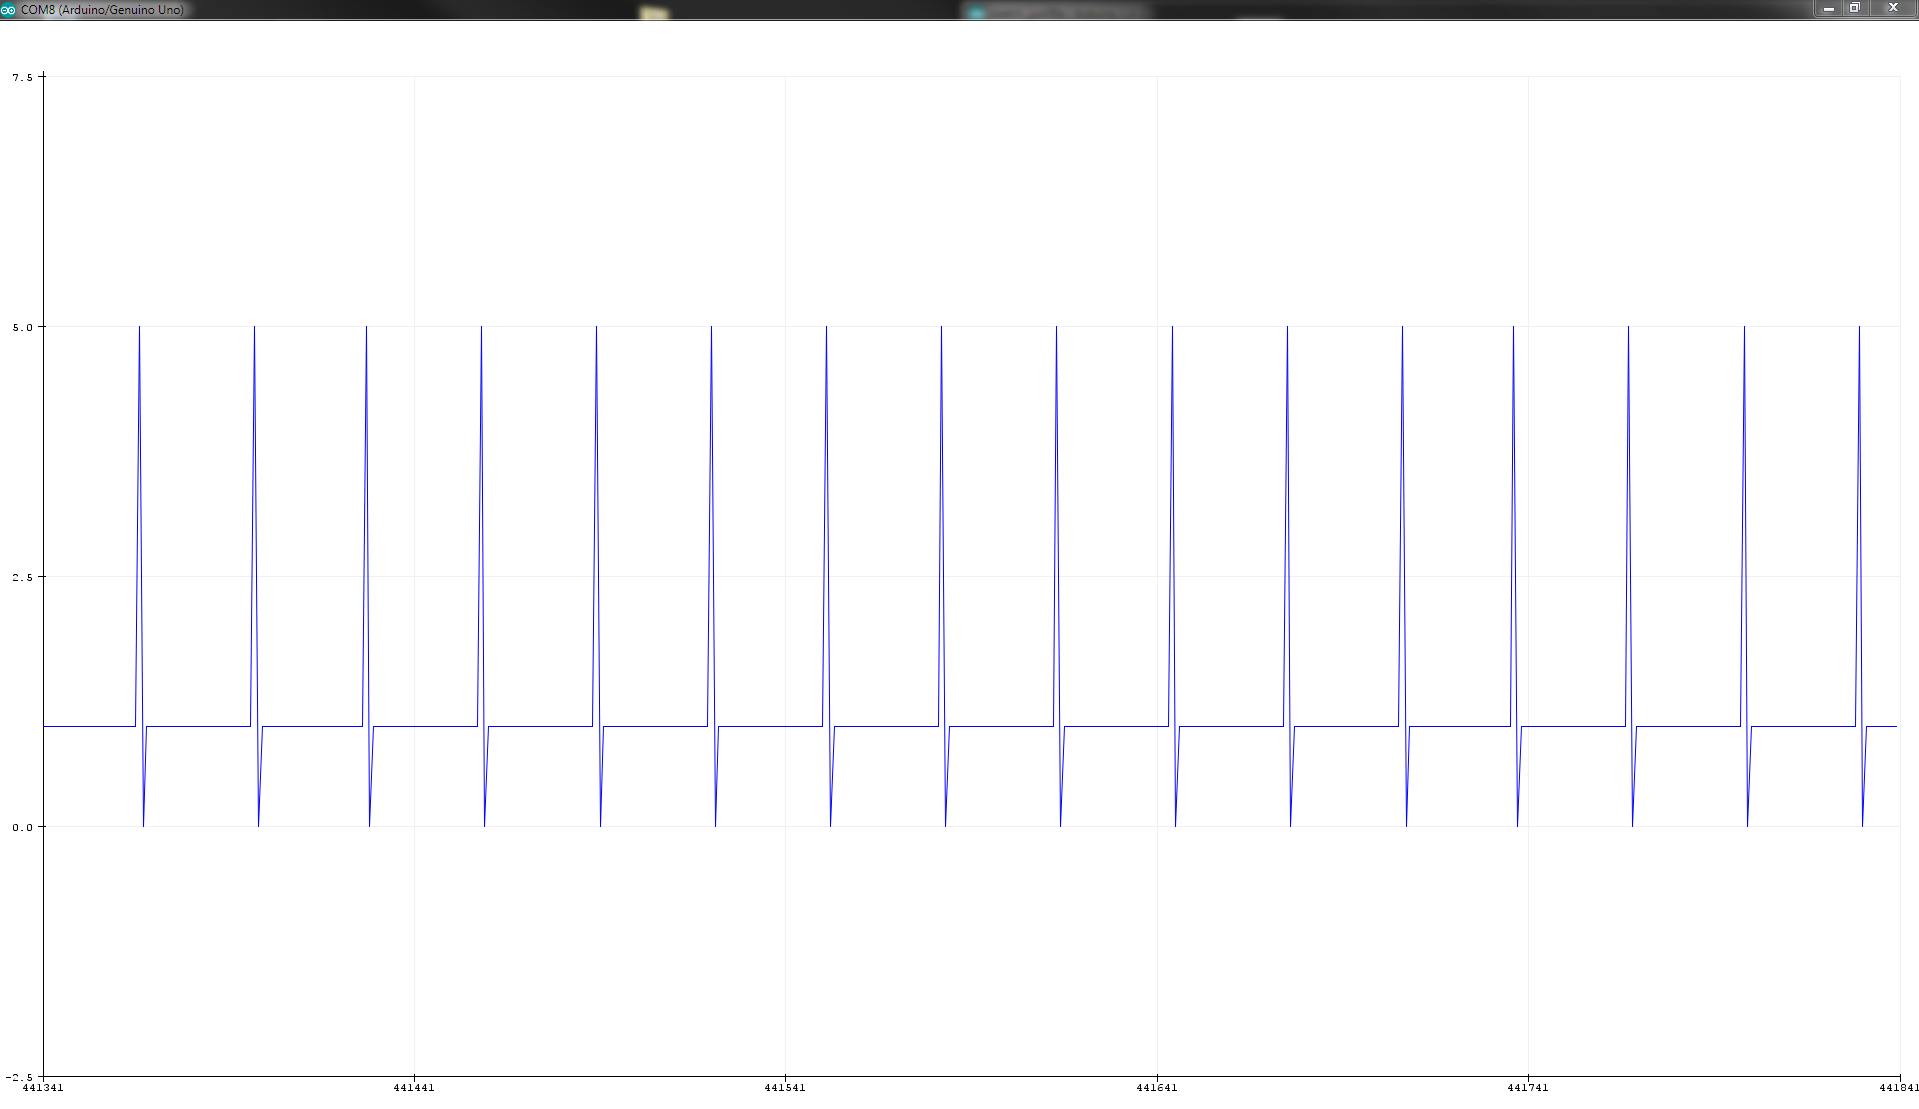
\includegraphics[width=0.9\textwidth]{images/chapter/03/self_made_interrupt_a1.png}
	\caption{Messerte des \ac{A1}}
	\label{fig:self_made_interrupt_a1}
\end{figure}

\subsection{Detektion der Unwucht}
\label{subsec:detektion_der_unwucht}

\subsubsection*{Theoretische Vorgehensweise}
Besitzt ein Propellerblatt eine Unwucht, erzeugt dieser deutlich spürbare Vibrationen am Motorblock.
Diese Vibrationen sollen mithilfe eines 3-Achsen-Sensors gemessen werden.
Je nach Auslenkung des Motorblockes kann hierdurch eine Unwucht detektiert werden.
Des Weiteren kann unter Berücksichtigung der Propellerdetektion, eine Unwuchtlokalisierung erfolgen. 

Zur Erzeugung einer Unwucht, werden wie in Abbildung \ref{fig:propeller-mit-unwucht} gezeigt, mehrere Propeller mit unterschiedlichen Gewichten, bzw. identischen Gewichten jedoch an unterschiedlichen Stellen, präpariert.
\begin{figure}[H]
	\centering
	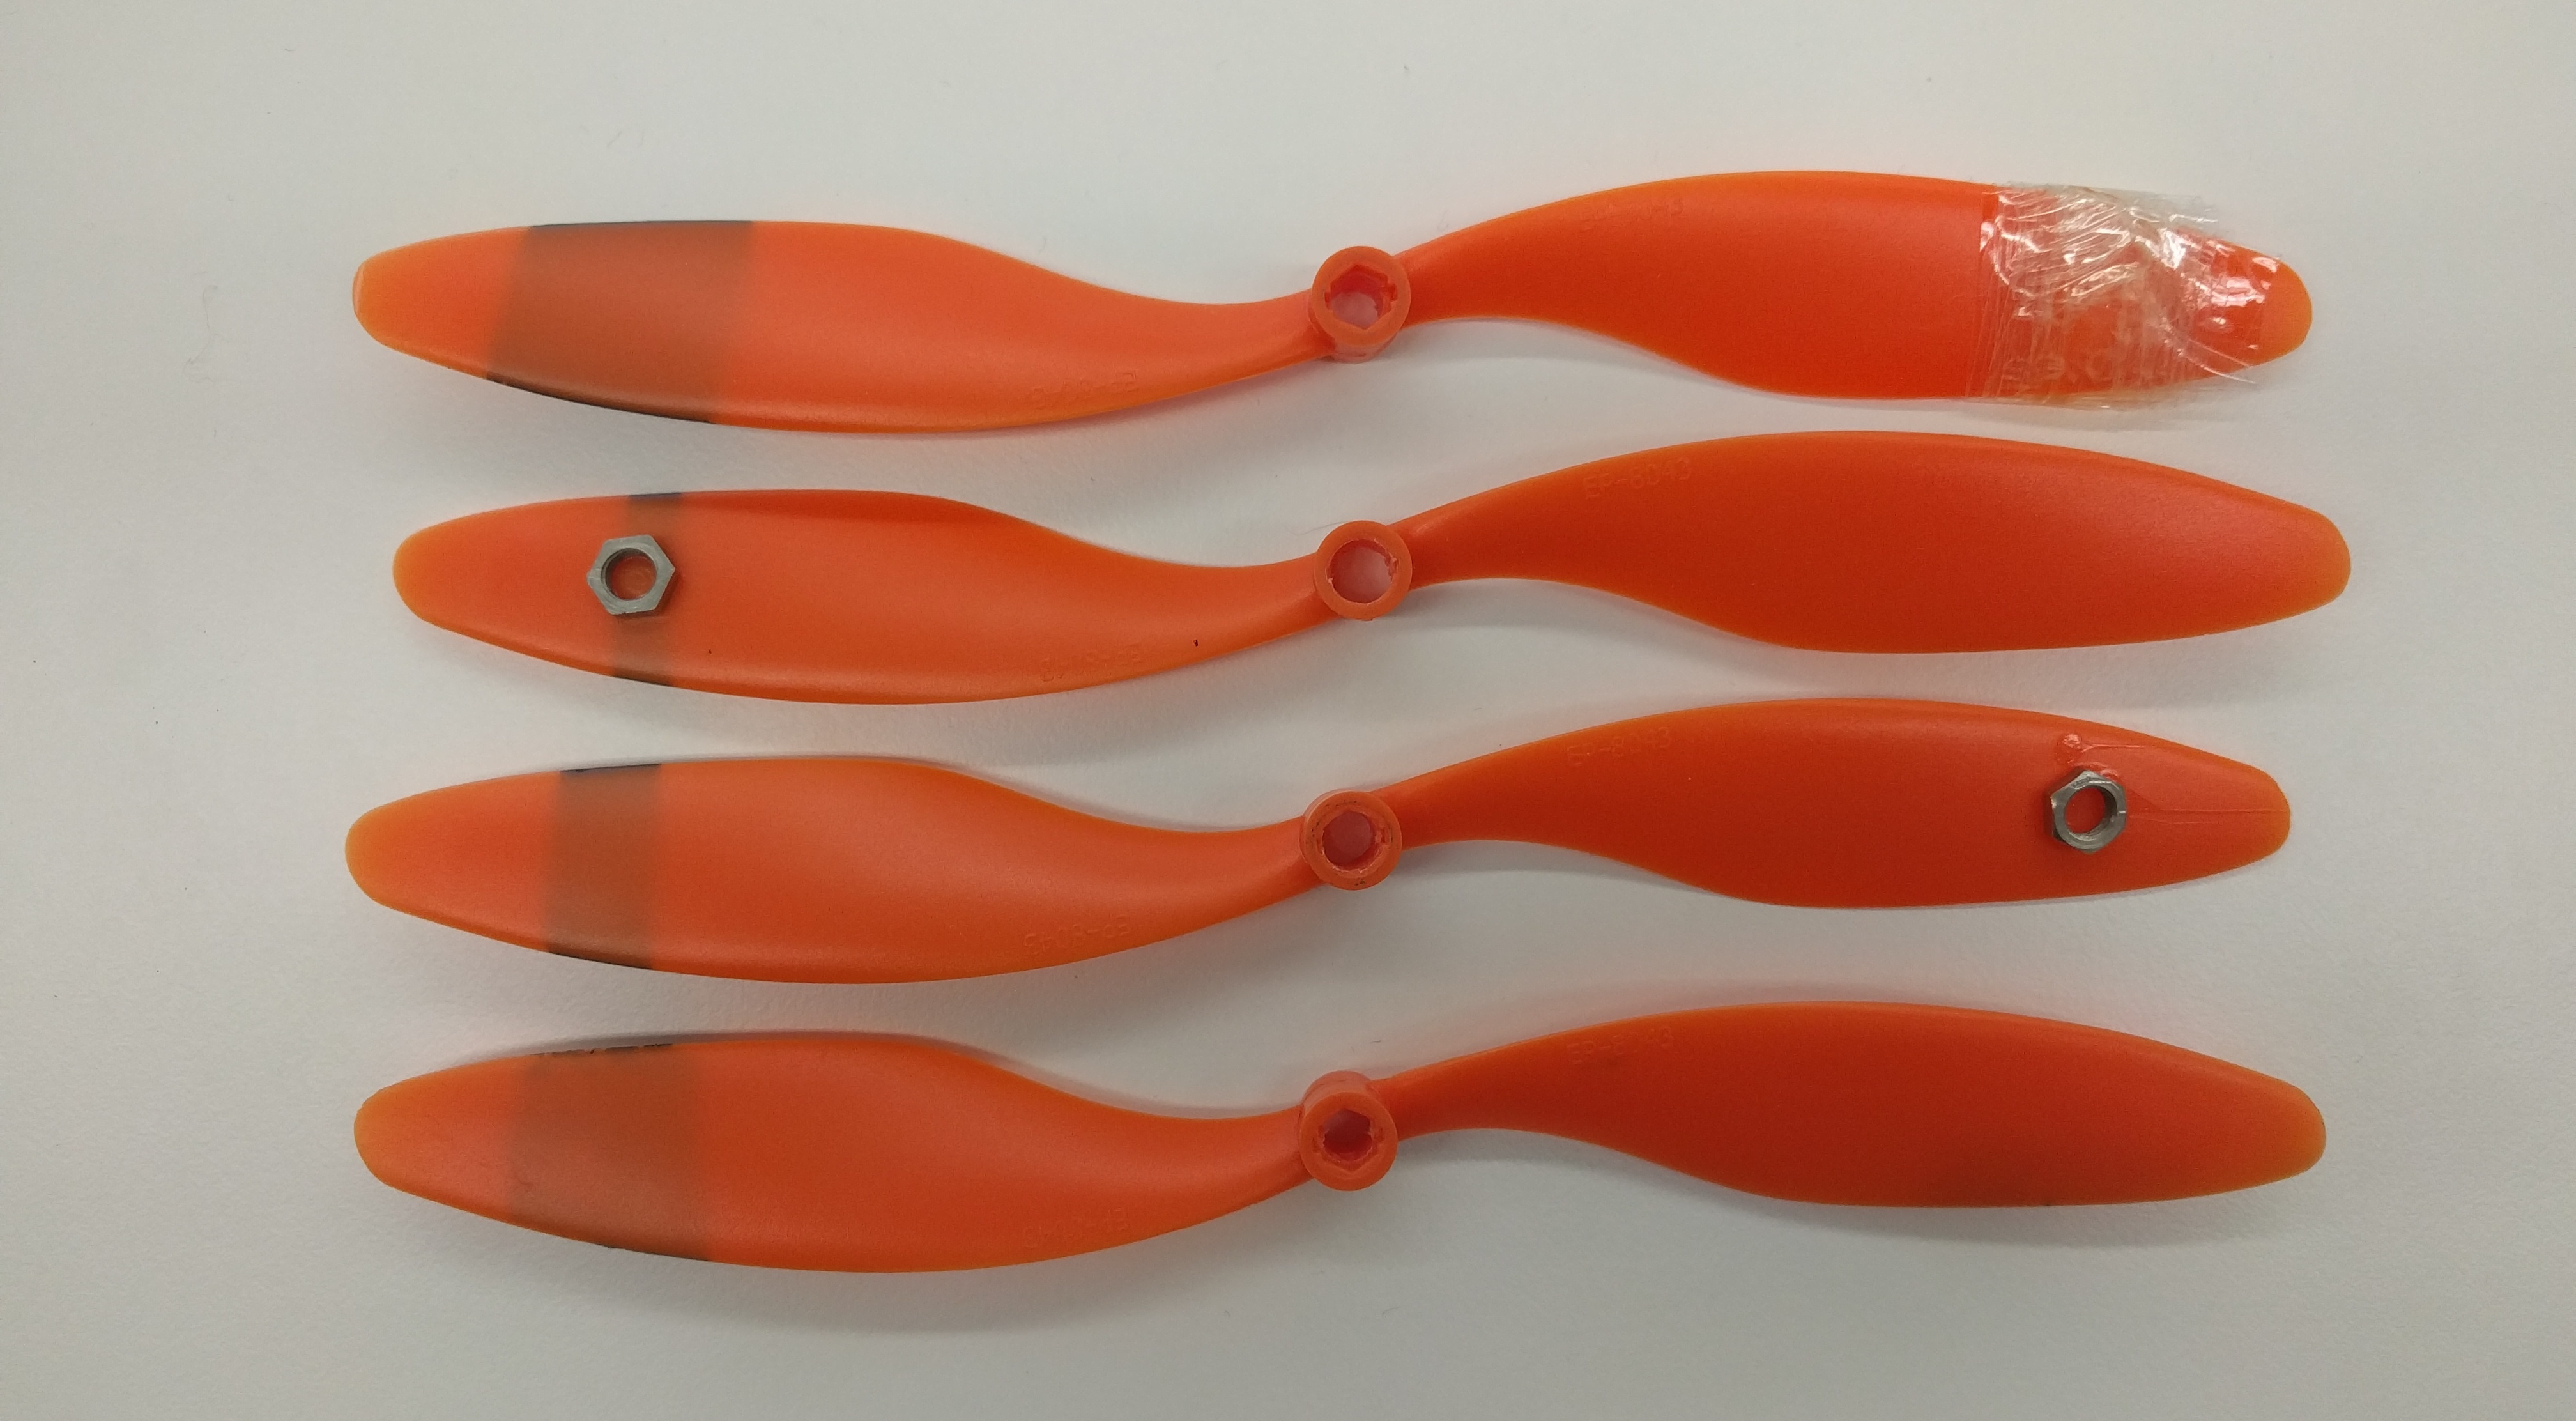
\includegraphics[width=0.9\textwidth]{images/chapter/03/propeller-mit-unwucht.png}
	\caption{Propeller mit unterschiedlichen Unwuchten}
	\label{fig:propeller-mit-unwucht}
\end{figure}

\subsubsection*{Sensortechnologie}
\label{subsec:unwucht_sensor}
Als 3-Achsen-Sensor soll der LSM9DS1 9-DOF Sensor von Adafruit eingesetzt werden.
\begin{figure}[H]
	\centering
	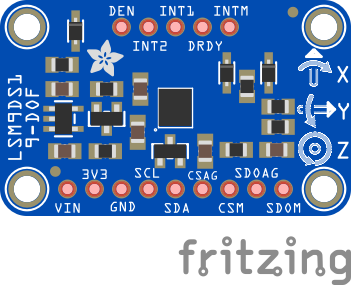
\includegraphics[width=5cm]{images/chapter/03/9-dof.png}
	\caption{Schematische Darstellung des verwendeten Sensors}
\end{figure}
Dieser ist mit 4 verschiedenen Sensoren ausgestattet:
\begin{itemize}
	\item Beschleunigungssensor (Beschleunigung des Sensors in drei Richtungen)
	\item Gyroskop (Ausrichtung des Sensors)
	\item Magnetometer (Lage in Abhängigkeit des Erdmagnetfeldes)
	\item Temperatursensor
\end{itemize}

\subsubsection*{Messung der Unwucht}
Wie bereits unter dem vorherigen Punkt beschrieben, existieren verschiedene Sensoren auf dem \ac{9-DOF}.
Für die Messung der Unwucht wird zunächst allerdings nur der Beschleunigungssensor eingesetzt.
Die von ihm gelieferten Werte zeigen am deutlichsten eine Verschiebung des Motorblockes, aufgrund von Vibrationen, an.

\begin{figure}[H]
	\centering
	\includegraphics[width=8cm]{images/chapter/03/measurement_arduino_a2.png}
	\caption{Ablaufdiagramm für die Unwuchtmessung am \ac{A2}}
	\label{fig:sequence_measure_a2}
\end{figure}

Für die erste Messreihenermittlung wurde das Programm von \ac{A2} auf den Ablauf programmiert, wie in Abbildung \ref{fig:sequence_measure_a2} dargestellt.
Hierbei wartet \ac{A2} auf einen Interrupt von \ac{A1} um mit der Unwuchtmessung zu beginnen.
Sobald ein weiterer Interrupt an \ac{A2} gesendet wird, kann davon ausgegangen werden, dass der Propeller eine vollständige Umdrehung absolviert hat und die Unwuchtmessung abgeschlossen werden kann.
Dieser erste Test soll zeigen, ob mögliche Muster in den Messwerten einer einzelnen Propellerumdrehung zu sehen sind.
Verwendet wird hierfür ein Propeller, dessen Unwucht auf der gleichen Seite, wie die Markierung ist.

Die aufgezeichneten Messwerte der einzelnen Messungen für diesen ersten Test, sind in zwei Tabellen dargestellt, welche jeweils drei Messergebnisse enthalten.
Tabelle \ref{tab:rounds_balance} enthält die Messergebnisse für einen Propeller ohne eigens erstellte Unwucht.

\begin{table}[H]
\centering
\resizebox{\textwidth}{!}{%
\begin{tabular}{l|llll|llll|llll}
\textbf{Messung} & \textbf{Zeit} & \textbf{X} & \textbf{Y} & \textbf{Z} & \textbf{Zeit} & \textbf{X} & \textbf{Y} & \textbf{Z} & \textbf{Zeit} & \textbf{X} & \textbf{Y} & \textbf{Z} \\
\hline
1       & 7    & 1,94  & 0,11  & 10,41 & 8    & 0,56  & -0,29 & 10,10 & 9    & 4,12  & 0,46  & 11,16 \\
2       & 15   & 2,10  & 0,86  & 10,61 & 16   & -0,24 & 0,08  & 9,54  & 17   & -0,34 & 0,39  & 9,26  \\
3       & 24   & -2,57 & -0,29 & 8,49  & 25   & -2,11 & -0,16 & 7,55  & 25   & 1,79  & -0,09 & 10,13
\end{tabular}%
}
\caption{Messergebnisse von Propellerumdrehungen ohne Unwucht}
\label{tab:rounds_balance}
\end{table}

Aus dieser Tabelle können mehrere Erkenntnisse gezogen werden.
Zunächst ist erkennbar, dass pro Messung (Zeit, X, Y, Z) nur drei Messpunkte aus dem Beschleunigungssensor gelesen werden konnten.
Außerdem weichen die Zeitpunkte um bis zu 2 \ac{ms} voneinander ab, an denen die Messergebnisse aus dem Sensor gelesen wurden.
Dies entspricht, bei der eingestellten Drehzahl des Motors von 2500 U/min, einer Verschiebung des räumlichen Messpunktes um 30$\,^\circ$.
Weiterhin sind Unstimmigkeiten zwischen den einzelnen Messreihen zu erkennen.
Ein Beispiel hierfür ist zwischen den ersten Beiden und der letzten Messreihe zu sehen.
Hierbei liegt der X-Wert der dritten Messung bei den ersten Beiden, trotz einer Zeitdifferenz von 1 \ac{ms}, bei ungefähr $2\;m/s^2$.
Der X-Wert der dritten Messreihe hingegen, steht mit einem Wert von $1,79\;m/s^2$ im genauen Gegenteil dazu.
Zuletzt fällt der Wert $19,60\;m/s^2$ häufig in den Messergebnissen auf.
Dies liegt an der eingestellten Messweite des Beschleunigungssensors, welche standardmäßig bei der zweifachen Erdbeschleunigung liegt.
Für die nachfolgenden Tests wurde diese auf die vierfache Erdbeschleunigung gesetzt.
Diese Erhöhung der Reichweite ist jedoch eine Verminderung der Präzision des Sensors geschuldet \cite{lsm9ds1_manual}, die jedoch keinen erkennbare Einfluss auf die Messung hat.

In Tabelle \ref{tab:rounds_imbalance} sind die Messergebnisse für den ersten Test mit einem unwuchtbehafteten Propeller enthalten.
Auffällig ist hierbei, die Existenz des vierten Messpunktes in allen drei Messreihen.
Dies scheint der Unwucht verschuldet zu sein, welche den Propeller langsamer drehen lässt, als ohne.
Trotz einer zusätzlichen Messung, sind die gleichen Inkonsistenzen zwischen den einzelnen Messreihen zu erkennen, wie in der Beschreibung der Tabelle \ref{tab:rounds_balance} bereits erwähnt.

\begin{table}[H]
\centering
\resizebox{\textwidth}{!}{%
\begin{tabular}{l|llll|llll|llll}
\textbf{Messung} & \textbf{Zeit} & \textbf{X} & \textbf{Y} & \textbf{Z} & \textbf{Zeit} & \textbf{X} & \textbf{Y} & \textbf{Z} & \textbf{Zeit} & \textbf{X} & \textbf{Y} & \textbf{Z} \\
\hline
1       & 7    & -17.49 & 0,83  & -0,60 & 7    & -14,92 & 1,27  & 0,83  & 8    & -18,98 & 0,88  & -1,78 \\
2       & 16   & -19,60 & -5,30 & -0,28 & 16   & -19,60 & -5,29 & -0,25 & 17   & -19,60  & -4,68 & 0,71  \\
3       & 25   & 19,60  & 4,02  & 19,60 & 25   & 19,60  & 2,24  & 19,60 & 25   & 19,60  & 2,72  & 19,60 \\
4       & 33   & -17,21 & 0,95  & -0,66 & 34   & 4,18   & 2,66  & 3,90  & 34   & 0,63   & 2,32  & 3,40 
\end{tabular}%
}
\caption{Messergebnisse von Propellerumdrehungen mit Unwucht}
\label{tab:rounds_imbalance}
\end{table}

Als Fazit des ersten Versuchs kann gezogen werden, dass eine Unwuchtlokalisierung an den Propellern aufgrund der teils großen Unstimmigkeiten zwischen den Messreihen mit diesem Vorgehen nicht möglich ist.
Eine Unwuchtdetektion hingegen, ist bereits realisierbar.
Zu erkennen ist dies an den zahlreichen Vorkommnissen von Maximalwerten in Tabelle \ref{tab:rounds_imbalance}, während die Tabelle \ref{tab:rounds_balance} hiervon keine enthält.

Aufgrund der prinzipellen Möglichkeit, Unwucht detektieren zu können, wird ein neuer Test gestartet.
Hierbei kommen zwei verschiedene Propeller zum Einsatz, die in Abbildung \ref{fig:test_two_propellers} betrachtet werden können.

\begin{figure}[H]
	\centering
	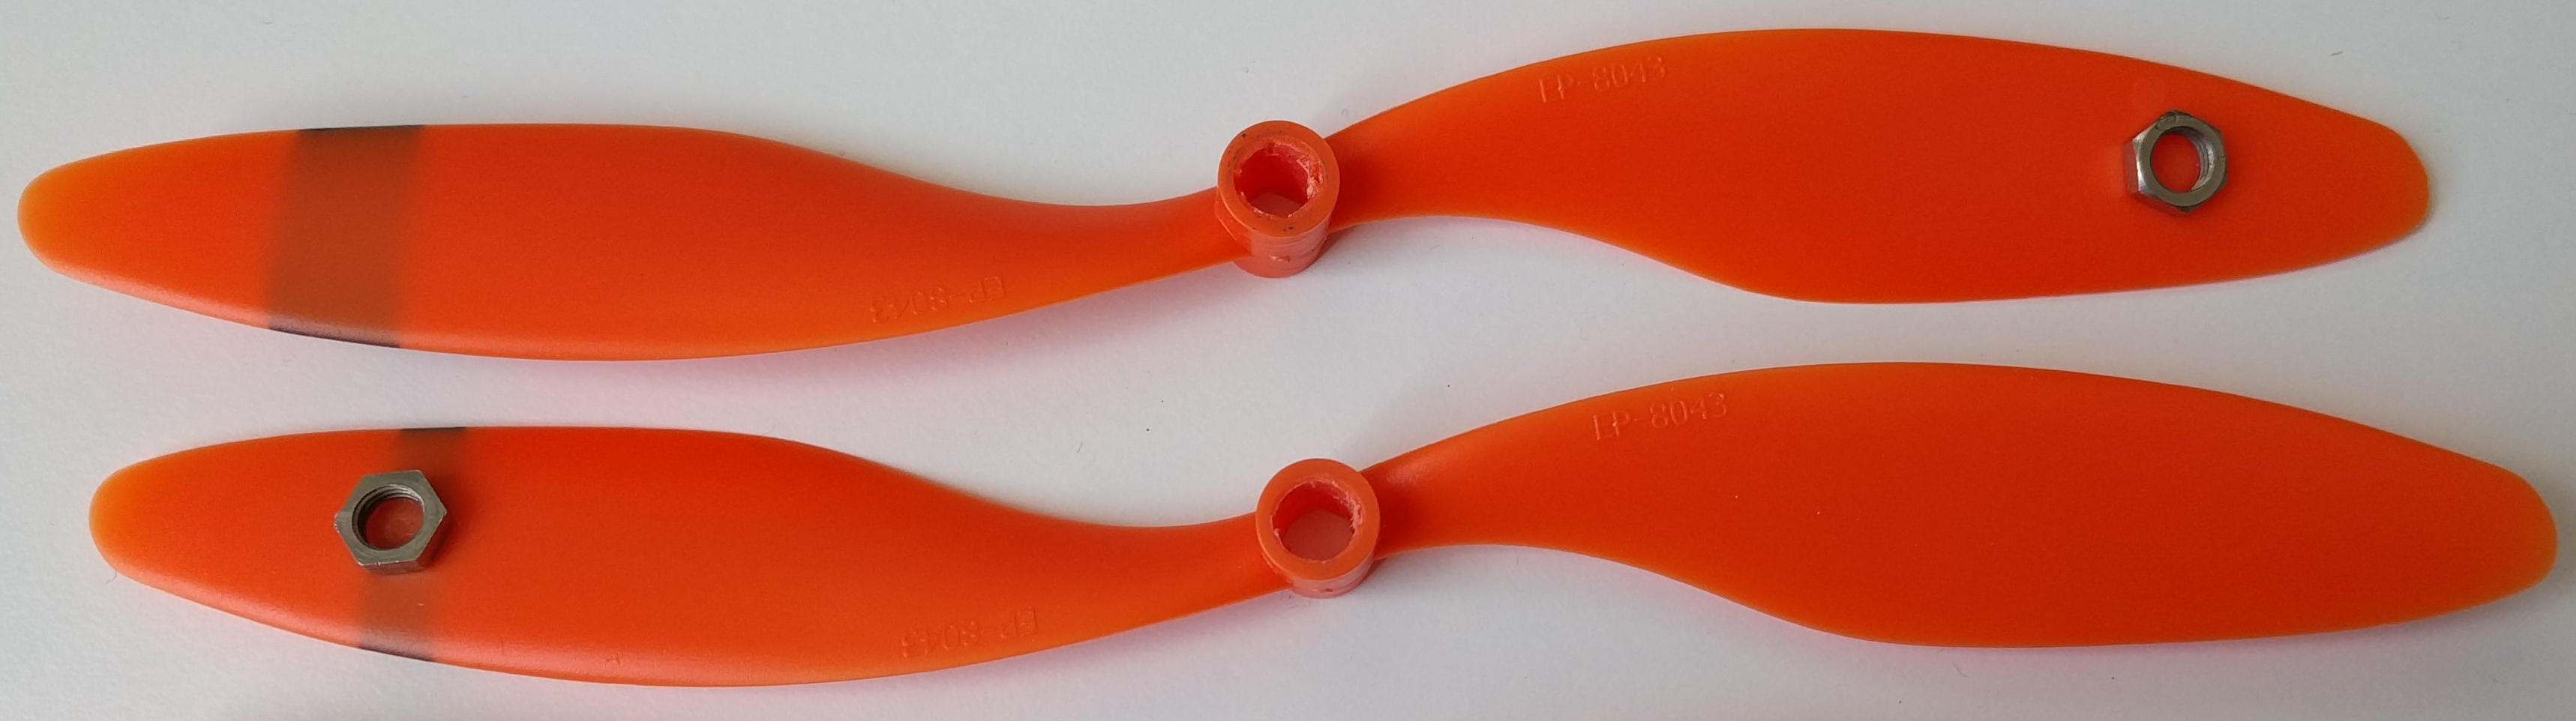
\includegraphics[width=8cm]{images/chapter/03/test_two_propellers.jpeg}
	\caption{Verwendete Propeller für den zweiten Test}
	\label{fig:test_two_propellers}
\end{figure}

Der erste Propeller besitzt eine Unwucht auf demselben Rotorblatt, an dem auch die Markierung existiert.
Die Unwucht des zweiten Propellers hingegen, ist auf dem Rotorblatt angebracht, welche keine Markierung besitzt.
Dieser Test soll zeigen, ob bestimmte charakteristische Messungwerte der jeweils eingesetzten Propeller zu sehen sind.
Bei einem erfolgreichen Testergebnis, kann aufgrund dieser ein Rückschluss auf den eingesetzten Propeller geschlossen werden.
Damit ist die Aussage über eine Unwuchtlokalisierung möglich.

Die Messergebnisse des zweiten Tests sind in Tabelle \ref{tab:imbalance_same_side} und in Tabelle \ref{tab:imbalance_other_side} auszugsweise dargestellt.
Die kompletten Messreihen können in Anhang unter dem Punkt Tabellen \ref{tab:imbalance_same_side-full} und \ref{tab:imbalance_other_side-full} eingesehen werden.

\begin{table}[H]
\centering
\resizebox{\textwidth}{!}{%
\begin{tabular}{lllllllllllll}
\textbf{Messung} & \textbf{Zeit} & \textbf{X} & \textbf{Y} & \textbf{Z} & \textbf{Zeit} & \textbf{X} & \textbf{Y} & \textbf{Z} & \textbf{Zeit} & \textbf{X} & \textbf{Y} & \textbf{Z} \\
\hline
1       & 3    & -1,95 & -2,94 & 9,76 & 7    & 27,69  & 0,88  & 22,27 & 11   & 26,13  & 4,14  & 19,55 \\
2       & 3    & -6,73 & -3,49 & 8,09 & 7    & 21,46  & -0,05 & 19,15 & 11   & 25,16  & 3,60  & 19,27 \\
3       & 3    & 0,44  & 2,35  & 8,12 & 7    & -20,35 & -0,27 & 0,47  & 11   & -20,78 & -2,42 & 1,55 
\end{tabular}%
}
\caption{Messergebnisse mit Unwucht auf Seite mit Markierung}
\label{tab:imbalance_same_side}
\end{table}

\begin{table}[H]
\centering
\resizebox{\textwidth}{!}{%
\begin{tabular}{lllllllllllll}
\textbf{Messung} & \textbf{Zeit} & \textbf{X} & \textbf{Y} & \textbf{Z} & \textbf{Zeit} & \textbf{X} & \textbf{Y} & \textbf{Z} & \textbf{Zeit} & \textbf{X} & \textbf{Y} & \textbf{Z} \\
\hline
1       & 3    & 0,10  & -2,01 & 11,81 & 7    & 26,25 & 1,73 & 21,20 & 12   & 24,31 & 3,88 & 17,53 \\
2       & 3    & -2,36 & -2,27 & 10,38 & 7    & 25,51 & 1,74 & 21,08 & 11   & 25,94 & 4,38 & 19,15 \\
3       & 3    & -1,89 & -1,87 & 10,43 & 7    & 26,03 & 1,21 & 20,58 & 11   & 27,78 & 4,24 & 19,98
\end{tabular}%
}
\caption{Messergebnisse mit Unwucht auf Seite ohne Markierung}
\label{tab:imbalance_other_side}
\end{table}

Die theoretische Vermutung ist, dass der Z-Wert sich bei den verschiedenen Propellerarten, jeweils entgegengesetzt verhält.
Dies ist begründet durch die Annahme, dass die Unwucht eine Auslenkung dieser Achse bewirkt, welche sich direkt Proportional mit der Lokalisation der Unwucht verhält.
Aus den Messergebnissen dieses Versuchs, kann diese Vermutung jedoch nicht bestätigt werden.
Es sind keinerlei charakteristische Messungen für die jeweiligen Propeller vorhanden, welche in allen Messreihen durchgehend vorkommen.

\subsubsection*{Probleme bei der Detektion}
Nachfolgende Probleme traten bei der Verwendung des Sensors auf:
- Das Auslesen der Sensordaten dauert zu lange. Es ist möglich 2-3 Messergebnisse (Variation hängt von Gewicht des Propellers ab) innerhalb einer Umdrehung (~20ms) des Propellers zu erhalten. Ein Versuch dieses Verhalten zu verbessern bestand darin die Verbindungsgeschwindigkeit zwischen \textit{Arduino} und Sensor zu erhöhen. Die Verbindung zwischen den beiden Geräten findet über die Schnittstelle I\textsuperscript{2}C im normalen Modus statt. Durch Manipulation der \textit{twi.h}, eine Header-Datei der Arduino-Bibliothek \textit{Wire.h}, welcher die Verbindungsparameter für die I\textsuperscript{2}C-Schnittstelle steuert, war es möglich die Verbindung im Fast-Mode zu betreiben. Damit wurde die Anzahl an Messergebnisse pro Umdrehung von 2-3 auf 3-5 Messungen erhöht. Dies ist aber weiterhin zu wenig um eine konkrete Entscheidung über die Lokalisation der Unwucht treffen zu können.
Es existiert eine weitere Möglichkeit den Sensor auf eine höhere Messrate zu bekommen, welche im Datenblatt jedoch nur sehr kurz und knapp erklärt ist. Hierbei ist es möglich das Gyroskop des Sensor abzuschalten und den Beschleunigungssensor mittels eines "Burst-Modus" (multiple reads) auszulesen. Den Sensor in diesen Modus zu setzen und auszulesen war allerdings aufgrund Mangel des technischen Verständnisses und der Datenblatterklärung nicht möglich.
Es kann davon ausgegangen werden, dass die benötigte Zeit für die Messung der Sensoren bei dem eingesetzten Sensor schon intern zu lange dauert. Die Empfehlung (für zukünftige Projekte ?) liegt daher auf dem Einsatz von anderen Sensoren, welche für diesen Einsatzzweck besser geeignet sind.
